% Options for packages loaded elsewhere
\PassOptionsToPackage{unicode}{hyperref}
\PassOptionsToPackage{hyphens}{url}
\PassOptionsToPackage{dvipsnames,svgnames,x11names}{xcolor}
%
\documentclass[
  11pt,
]{article}

\usepackage{amsmath,amssymb}
\usepackage{iftex}
\ifPDFTeX
  \usepackage[T1]{fontenc}
  \usepackage[utf8]{inputenc}
  \usepackage{textcomp} % provide euro and other symbols
\else % if luatex or xetex
  \usepackage{unicode-math}
  \defaultfontfeatures{Scale=MatchLowercase}
  \defaultfontfeatures[\rmfamily]{Ligatures=TeX,Scale=1}
\fi
\usepackage{lmodern}
\ifPDFTeX\else  
    % xetex/luatex font selection
    \setmainfont[]{Times New Roman}
\fi
% Use upquote if available, for straight quotes in verbatim environments
\IfFileExists{upquote.sty}{\usepackage{upquote}}{}
\IfFileExists{microtype.sty}{% use microtype if available
  \usepackage[]{microtype}
  \UseMicrotypeSet[protrusion]{basicmath} % disable protrusion for tt fonts
}{}
\makeatletter
\@ifundefined{KOMAClassName}{% if non-KOMA class
  \IfFileExists{parskip.sty}{%
    \usepackage{parskip}
  }{% else
    \setlength{\parindent}{0pt}
    \setlength{\parskip}{6pt plus 2pt minus 1pt}}
}{% if KOMA class
  \KOMAoptions{parskip=half}}
\makeatother
\usepackage{xcolor}
\usepackage[margin=1in]{geometry}
\setlength{\emergencystretch}{3em} % prevent overfull lines
\setcounter{secnumdepth}{-\maxdimen} % remove section numbering
% Make \paragraph and \subparagraph free-standing
\makeatletter
\ifx\paragraph\undefined\else
  \let\oldparagraph\paragraph
  \renewcommand{\paragraph}{
    \@ifstar
      \xxxParagraphStar
      \xxxParagraphNoStar
  }
  \newcommand{\xxxParagraphStar}[1]{\oldparagraph*{#1}\mbox{}}
  \newcommand{\xxxParagraphNoStar}[1]{\oldparagraph{#1}\mbox{}}
\fi
\ifx\subparagraph\undefined\else
  \let\oldsubparagraph\subparagraph
  \renewcommand{\subparagraph}{
    \@ifstar
      \xxxSubParagraphStar
      \xxxSubParagraphNoStar
  }
  \newcommand{\xxxSubParagraphStar}[1]{\oldsubparagraph*{#1}\mbox{}}
  \newcommand{\xxxSubParagraphNoStar}[1]{\oldsubparagraph{#1}\mbox{}}
\fi
\makeatother

\usepackage{color}
\usepackage{fancyvrb}
\newcommand{\VerbBar}{|}
\newcommand{\VERB}{\Verb[commandchars=\\\{\}]}
\DefineVerbatimEnvironment{Highlighting}{Verbatim}{commandchars=\\\{\}}
% Add ',fontsize=\small' for more characters per line
\usepackage{framed}
\definecolor{shadecolor}{RGB}{241,243,245}
\newenvironment{Shaded}{\begin{snugshade}}{\end{snugshade}}
\newcommand{\AlertTok}[1]{\textcolor[rgb]{0.68,0.00,0.00}{#1}}
\newcommand{\AnnotationTok}[1]{\textcolor[rgb]{0.37,0.37,0.37}{#1}}
\newcommand{\AttributeTok}[1]{\textcolor[rgb]{0.40,0.45,0.13}{#1}}
\newcommand{\BaseNTok}[1]{\textcolor[rgb]{0.68,0.00,0.00}{#1}}
\newcommand{\BuiltInTok}[1]{\textcolor[rgb]{0.00,0.23,0.31}{#1}}
\newcommand{\CharTok}[1]{\textcolor[rgb]{0.13,0.47,0.30}{#1}}
\newcommand{\CommentTok}[1]{\textcolor[rgb]{0.37,0.37,0.37}{#1}}
\newcommand{\CommentVarTok}[1]{\textcolor[rgb]{0.37,0.37,0.37}{\textit{#1}}}
\newcommand{\ConstantTok}[1]{\textcolor[rgb]{0.56,0.35,0.01}{#1}}
\newcommand{\ControlFlowTok}[1]{\textcolor[rgb]{0.00,0.23,0.31}{\textbf{#1}}}
\newcommand{\DataTypeTok}[1]{\textcolor[rgb]{0.68,0.00,0.00}{#1}}
\newcommand{\DecValTok}[1]{\textcolor[rgb]{0.68,0.00,0.00}{#1}}
\newcommand{\DocumentationTok}[1]{\textcolor[rgb]{0.37,0.37,0.37}{\textit{#1}}}
\newcommand{\ErrorTok}[1]{\textcolor[rgb]{0.68,0.00,0.00}{#1}}
\newcommand{\ExtensionTok}[1]{\textcolor[rgb]{0.00,0.23,0.31}{#1}}
\newcommand{\FloatTok}[1]{\textcolor[rgb]{0.68,0.00,0.00}{#1}}
\newcommand{\FunctionTok}[1]{\textcolor[rgb]{0.28,0.35,0.67}{#1}}
\newcommand{\ImportTok}[1]{\textcolor[rgb]{0.00,0.46,0.62}{#1}}
\newcommand{\InformationTok}[1]{\textcolor[rgb]{0.37,0.37,0.37}{#1}}
\newcommand{\KeywordTok}[1]{\textcolor[rgb]{0.00,0.23,0.31}{\textbf{#1}}}
\newcommand{\NormalTok}[1]{\textcolor[rgb]{0.00,0.23,0.31}{#1}}
\newcommand{\OperatorTok}[1]{\textcolor[rgb]{0.37,0.37,0.37}{#1}}
\newcommand{\OtherTok}[1]{\textcolor[rgb]{0.00,0.23,0.31}{#1}}
\newcommand{\PreprocessorTok}[1]{\textcolor[rgb]{0.68,0.00,0.00}{#1}}
\newcommand{\RegionMarkerTok}[1]{\textcolor[rgb]{0.00,0.23,0.31}{#1}}
\newcommand{\SpecialCharTok}[1]{\textcolor[rgb]{0.37,0.37,0.37}{#1}}
\newcommand{\SpecialStringTok}[1]{\textcolor[rgb]{0.13,0.47,0.30}{#1}}
\newcommand{\StringTok}[1]{\textcolor[rgb]{0.13,0.47,0.30}{#1}}
\newcommand{\VariableTok}[1]{\textcolor[rgb]{0.07,0.07,0.07}{#1}}
\newcommand{\VerbatimStringTok}[1]{\textcolor[rgb]{0.13,0.47,0.30}{#1}}
\newcommand{\WarningTok}[1]{\textcolor[rgb]{0.37,0.37,0.37}{\textit{#1}}}

\providecommand{\tightlist}{%
  \setlength{\itemsep}{0pt}\setlength{\parskip}{0pt}}\usepackage{longtable,booktabs,array}
\usepackage{calc} % for calculating minipage widths
% Correct order of tables after \paragraph or \subparagraph
\usepackage{etoolbox}
\makeatletter
\patchcmd\longtable{\par}{\if@noskipsec\mbox{}\fi\par}{}{}
\makeatother
% Allow footnotes in longtable head/foot
\IfFileExists{footnotehyper.sty}{\usepackage{footnotehyper}}{\usepackage{footnote}}
\makesavenoteenv{longtable}
\usepackage{graphicx}
\makeatletter
\newsavebox\pandoc@box
\newcommand*\pandocbounded[1]{% scales image to fit in text height/width
  \sbox\pandoc@box{#1}%
  \Gscale@div\@tempa{\textheight}{\dimexpr\ht\pandoc@box+\dp\pandoc@box\relax}%
  \Gscale@div\@tempb{\linewidth}{\wd\pandoc@box}%
  \ifdim\@tempb\p@<\@tempa\p@\let\@tempa\@tempb\fi% select the smaller of both
  \ifdim\@tempa\p@<\p@\scalebox{\@tempa}{\usebox\pandoc@box}%
  \else\usebox{\pandoc@box}%
  \fi%
}
% Set default figure placement to htbp
\def\fps@figure{htbp}
\makeatother

\makeatletter
\@ifpackageloaded{caption}{}{\usepackage{caption}}
\AtBeginDocument{%
\ifdefined\contentsname
  \renewcommand*\contentsname{Table of contents}
\else
  \newcommand\contentsname{Table of contents}
\fi
\ifdefined\listfigurename
  \renewcommand*\listfigurename{List of Figures}
\else
  \newcommand\listfigurename{List of Figures}
\fi
\ifdefined\listtablename
  \renewcommand*\listtablename{List of Tables}
\else
  \newcommand\listtablename{List of Tables}
\fi
\ifdefined\figurename
  \renewcommand*\figurename{Figure}
\else
  \newcommand\figurename{Figure}
\fi
\ifdefined\tablename
  \renewcommand*\tablename{Table}
\else
  \newcommand\tablename{Table}
\fi
}
\@ifpackageloaded{float}{}{\usepackage{float}}
\floatstyle{ruled}
\@ifundefined{c@chapter}{\newfloat{codelisting}{h}{lop}}{\newfloat{codelisting}{h}{lop}[chapter]}
\floatname{codelisting}{Listing}
\newcommand*\listoflistings{\listof{codelisting}{List of Listings}}
\makeatother
\makeatletter
\makeatother
\makeatletter
\@ifpackageloaded{caption}{}{\usepackage{caption}}
\@ifpackageloaded{subcaption}{}{\usepackage{subcaption}}
\makeatother

\usepackage{bookmark}

\IfFileExists{xurl.sty}{\usepackage{xurl}}{} % add URL line breaks if available
\urlstyle{same} % disable monospaced font for URLs
\hypersetup{
  pdftitle={Sydney Beach Quality and Safety Assessment Report},
  pdfauthor={Jingyi Wang},
  colorlinks=true,
  linkcolor={blue},
  filecolor={Maroon},
  citecolor={Blue},
  urlcolor={Blue},
  pdfcreator={LaTeX via pandoc}}


\title{Sydney Beach Quality and Safety Assessment Report}
\author{Jingyi Wang}
\date{}

\begin{document}
\maketitle

\renewcommand*\contentsname{Table of contents}
{
\hypersetup{linkcolor=}
\setcounter{tocdepth}{3}
\tableofcontents
}

\subsection{Load Library}\label{load-library}

\begin{Shaded}
\begin{Highlighting}[]
\FunctionTok{library}\NormalTok{(tidyverse)}
\FunctionTok{library}\NormalTok{(viridis)}
\FunctionTok{library}\NormalTok{(viridisLite)}
\FunctionTok{library}\NormalTok{(knitr)}
\end{Highlighting}
\end{Shaded}

\subsection{Dataset Description}\label{dataset-description}

\begin{Shaded}
\begin{Highlighting}[]
\NormalTok{water\_quality }\OtherTok{\textless{}{-}}\NormalTok{ readr}\SpecialCharTok{::}\FunctionTok{read\_csv}\NormalTok{(}\StringTok{\textquotesingle{}https://raw.githubusercontent.com/rfordatascience/tidytuesday/main/data/2025/2025{-}05{-}20/water\_quality.csv\textquotesingle{}}\NormalTok{)}
\NormalTok{weather }\OtherTok{\textless{}{-}}\NormalTok{ readr}\SpecialCharTok{::}\FunctionTok{read\_csv}\NormalTok{(}\StringTok{\textquotesingle{}https://raw.githubusercontent.com/rfordatascience/tidytuesday/main/data/2025/2025{-}05{-}20/weather.csv\textquotesingle{}}\NormalTok{)}
\end{Highlighting}
\end{Shaded}

\begin{Shaded}
\begin{Highlighting}[]
\NormalTok{start\_date }\OtherTok{\textless{}{-}} \FunctionTok{as.Date}\NormalTok{(}\StringTok{"2015{-}04{-}28"}\NormalTok{, }\AttributeTok{tz =}\StringTok{"Australia/Sydney"}\NormalTok{)}
\NormalTok{end\_date }\OtherTok{\textless{}{-}} \FunctionTok{as.Date}\NormalTok{(}\StringTok{"2025{-}04{-}28"}\NormalTok{, }\AttributeTok{tz =}\StringTok{"Australia/Sydney"}\NormalTok{)}

\NormalTok{water\_quality }\OtherTok{\textless{}{-}}\NormalTok{ water\_quality }\SpecialCharTok{\%\textgreater{}\%}
  \FunctionTok{filter}\NormalTok{(date }\SpecialCharTok{\textgreater{}=}\NormalTok{ start\_date }\SpecialCharTok{\&}\NormalTok{ date }\SpecialCharTok{\textless{}=}\NormalTok{ end\_date)}

\NormalTok{weather }\OtherTok{\textless{}{-}}\NormalTok{ weather }\SpecialCharTok{\%\textgreater{}\%}
  \FunctionTok{filter}\NormalTok{(date }\SpecialCharTok{\textgreater{}=}\NormalTok{ start\_date }\SpecialCharTok{\&}\NormalTok{ date }\SpecialCharTok{\textless{}=}\NormalTok{ end\_date)}
\end{Highlighting}
\end{Shaded}

The dataset utilized in this analysis originates from the TidyTuesday
project, specifically the release dated May 20, 2025. It encompasses two
primary components:

\begin{itemize}
\tightlist
\item
  Water Quality Data
\end{itemize}

This dataset comprises measurements of enterococci levels, expressed in
colony-forming units per 100 milliliters (CFU/100ml), collected from
various beaches across New South Wales, Australia.

\begin{itemize}
\tightlist
\item
  Weather Data
\end{itemize}

This dataset includes meteorological information.

\subsection{Executive Summary}\label{executive-summary}

This report investigates water pollution at public beaches by analysing
enterococci levels using environmental and weather data. The findings
show that several beaches have extremely high average pollution levels,
which poses serious health risks to swimmers. Moreover, enterococci
concentrations were significantly higher after rainfall, which suggests
that rain events are a strong predictor of poor water quality. We
recommend regular monitoring and public reporting of water quality,
especially after heavy rainfall.

\subsection{Introduction}\label{introduction}

Sydney's beaches are popular swimming spots, but water quality issues
sometimes occur. This report analyzes 10 years (2015-2025) of water test
data from beaches and weather data, originally collected by the
TidyTuesday project. We focus on Enterococci bacteria levels, which
indicate potential health risks.

Beach water quality is significant for health and tourism. Poor water
conditions can cause illness and reduce the number of visitors. This
analysis helps us understand two key questions:

\begin{itemize}
\tightlist
\item
  Which beaches have the worst water quality?
\item
  When do problems typically occur particularly after rainfall?
\end{itemize}

By using data science tools, we aim to give clear and useful insights.
Our goal is to support better decisions for beach safety and
environmental protection.

\subsection{Methodology}\label{methodology}

In this project, we aim to find which beaches have the worst water
quality in Sydney and whether the water quality becomes worse after
rainfall. We use two datasets: \texttt{water\_quality} and
\texttt{weather}. The water quality dataset records enterococci bacteria
levels in colony forming units (CFU) per 100 millilitres of water,
temperature, and conductivity at different swim sites. The weather
dataset provides daily rainfall data.

First, we calculate the average enterococci level for each beach
(swim\_site) to identify the most polluted beaches. We use a bar chart
(Figure~\ref{fig-bar_chart}) to show the top 10 beaches with the highest
average pollution levels.

\begin{Shaded}
\begin{Highlighting}[]
\NormalTok{top\_beaches }\OtherTok{\textless{}{-}}\NormalTok{ water\_quality }\SpecialCharTok{\%\textgreater{}\%}
  \FunctionTok{group\_by}\NormalTok{(swim\_site) }\SpecialCharTok{\%\textgreater{}\%}
  \FunctionTok{summarise}\NormalTok{(}\AttributeTok{avg\_enterococci =} \FunctionTok{mean}\NormalTok{(enterococci\_cfu\_100ml, }\AttributeTok{na.rm =} \ConstantTok{TRUE}\NormalTok{)) }\SpecialCharTok{\%\textgreater{}\%}
  \FunctionTok{arrange}\NormalTok{(}\FunctionTok{desc}\NormalTok{(avg\_enterococci)) }\SpecialCharTok{\%\textgreater{}\%}
  \FunctionTok{slice}\NormalTok{(}\DecValTok{1}\SpecialCharTok{:}\DecValTok{10}\NormalTok{)}
\end{Highlighting}
\end{Shaded}

\begin{figure}

\centering{

\pandocbounded{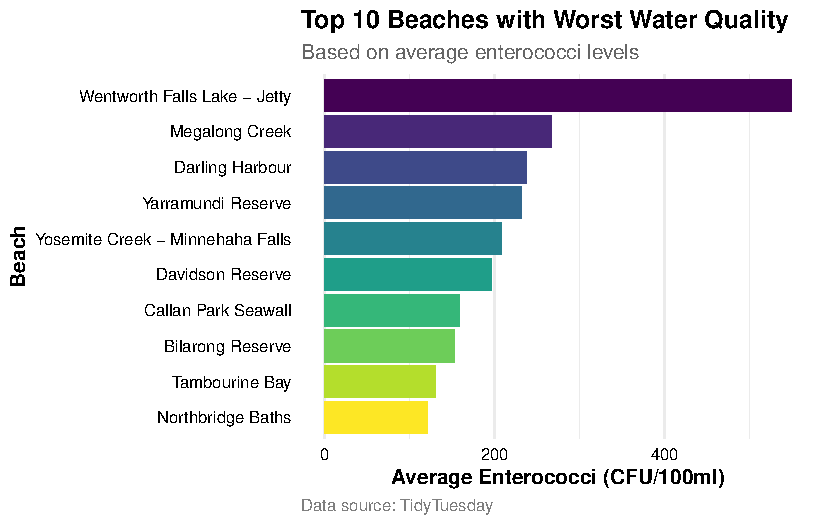
\includegraphics[keepaspectratio]{report-Jing_files/figure-pdf/fig-bar_chart-1.pdf}}

}

\caption{\label{fig-bar_chart}Top 10 Beaches with Worst Water Quality}

\end{figure}%

Second, we explore the relationship between rainfall and water quality.
We merge the two datasets by date and then group the data by rainfall
level (0 mm, 0--10 mm, \textgreater10 mm). We create a
table(Table~\ref{tbl-rain_table}) showing the average enterococci count
in each rainfall group. We also make a boxplot to show the distribution
of bacteria levels across these groups. Due to extreme values and some
zeros in enterococci counts, a log10 transformation was applied to
improve the visibility of the boxplot(Figure~\ref{fig-boxplot}).

\begin{Shaded}
\begin{Highlighting}[]
\CommentTok{\# In weather dataset, both latitude and longitude have only unique values.}
\NormalTok{weather }\OtherTok{\textless{}{-}}\NormalTok{ weather }\SpecialCharTok{\%\textgreater{}\%}
  \FunctionTok{select}\NormalTok{(}\SpecialCharTok{{-}}\NormalTok{latitude, }\SpecialCharTok{{-}}\NormalTok{longitude)}

\CommentTok{\# Merge water and weather datasets by date}
\NormalTok{water\_weather }\OtherTok{\textless{}{-}}\NormalTok{ water\_quality }\SpecialCharTok{\%\textgreater{}\%}
  \FunctionTok{left\_join}\NormalTok{(weather, }\AttributeTok{by =} \StringTok{"date"}\NormalTok{)}
\end{Highlighting}
\end{Shaded}

\begin{Shaded}
\begin{Highlighting}[]
\NormalTok{water\_weather }\OtherTok{\textless{}{-}}\NormalTok{ water\_weather }\SpecialCharTok{\%\textgreater{}\%}
  \FunctionTok{mutate}\NormalTok{(}\AttributeTok{rain\_group =} \FunctionTok{case\_when}\NormalTok{(}
\NormalTok{    precipitation\_mm }\SpecialCharTok{==} \DecValTok{0} \SpecialCharTok{\textasciitilde{}} \StringTok{"0 mm"}\NormalTok{,}
\NormalTok{    precipitation\_mm }\SpecialCharTok{\textless{}=} \DecValTok{10} \SpecialCharTok{\textasciitilde{}} \StringTok{"0–10 mm"}\NormalTok{,}
    \ConstantTok{TRUE} \SpecialCharTok{\textasciitilde{}} \StringTok{"\textgreater{}10 mm"}
\NormalTok{  ))}
\end{Highlighting}
\end{Shaded}

\begin{Shaded}
\begin{Highlighting}[]
\NormalTok{rain\_table }\OtherTok{\textless{}{-}}\NormalTok{ water\_weather }\SpecialCharTok{\%\textgreater{}\%}
  \FunctionTok{group\_by}\NormalTok{(rain\_group) }\SpecialCharTok{\%\textgreater{}\%}
  \FunctionTok{summarise}\NormalTok{(}\AttributeTok{mean\_enterococci =} \FunctionTok{mean}\NormalTok{(enterococci\_cfu\_100ml, }\AttributeTok{na.rm =} \ConstantTok{TRUE}\NormalTok{))}
\FunctionTok{kable}\NormalTok{(rain\_table)}
\end{Highlighting}
\end{Shaded}

\begin{longtable}[]{@{}lr@{}}

\caption{\label{tbl-rain_table}Average Enterococci by Rain Group}

\tabularnewline

\toprule\noalign{}
rain\_group & mean\_enterococci \\
\midrule\noalign{}
\endhead
\bottomrule\noalign{}
\endlastfoot
0 mm & 17.64191 \\
0--10 mm & 52.71743 \\
\textgreater10 mm & 167.10027 \\

\end{longtable}

\begin{Shaded}
\begin{Highlighting}[]
\FunctionTok{ggplot}\NormalTok{(water\_weather, }
       \FunctionTok{aes}\NormalTok{(}\AttributeTok{x =}\NormalTok{ rain\_group, }
           \AttributeTok{y =}\NormalTok{ enterococci\_cfu\_100ml, }
           \AttributeTok{fill =}\NormalTok{ rain\_group)) }\SpecialCharTok{+}  
  \FunctionTok{geom\_boxplot}\NormalTok{(}
    \AttributeTok{width =} \FloatTok{0.6}\NormalTok{,                }
    \AttributeTok{color =} \StringTok{"black"}\NormalTok{,            }
    \AttributeTok{size =} \FloatTok{0.5}\NormalTok{,                 }
    \AttributeTok{outlier.alpha =} \FloatTok{0.5}   \CommentTok{\# Outlier transparency}
\NormalTok{  ) }\SpecialCharTok{+}
  \FunctionTok{scale\_y\_log10}\NormalTok{() }\SpecialCharTok{+}
  \FunctionTok{scale\_fill\_manual}\NormalTok{(}
    \AttributeTok{values =} \FunctionTok{c}\NormalTok{(}\StringTok{"0 mm"} \OtherTok{=} \StringTok{"\#FDE725"}\NormalTok{,    }
               \StringTok{"0–10 mm"} \OtherTok{=} \StringTok{"\#7AD151"}\NormalTok{,}
               \StringTok{"\textgreater{}10 mm"} \OtherTok{=} \StringTok{"\#31688E"}\NormalTok{), }
    \AttributeTok{breaks =} \FunctionTok{c}\NormalTok{(}\StringTok{"0 mm"}\NormalTok{, }\StringTok{"0–10 mm"}\NormalTok{, }\StringTok{"\textgreater{}10 mm"}\NormalTok{)) }\SpecialCharTok{+}
  \FunctionTok{labs}\NormalTok{(}
    \AttributeTok{title =} \StringTok{"Enterococci Levels by Rainfall Group"}\NormalTok{,}
    \AttributeTok{subtitle =} \StringTok{"Log{-}transformed bacteria concentration (CFU/100ml)"}\NormalTok{,}
    \AttributeTok{x =} \StringTok{"Rainfall Group"}\NormalTok{,}
    \AttributeTok{y =} \StringTok{"Enterococci (CFU/100ml, log10)"}\NormalTok{,}
    \AttributeTok{caption =} \StringTok{"Color intensity reflects rainfall amount. Darker colors indicate higher rainfall."}
\NormalTok{  ) }\SpecialCharTok{+}
  \FunctionTok{theme\_minimal}\NormalTok{(}\AttributeTok{base\_size =} \DecValTok{10}\NormalTok{) }\SpecialCharTok{+}
  \FunctionTok{theme}\NormalTok{(}
    \AttributeTok{plot.title =} \FunctionTok{element\_text}\NormalTok{(}\AttributeTok{face =} \StringTok{"bold"}\NormalTok{, }\AttributeTok{size =} \DecValTok{12}\NormalTok{),}
    \AttributeTok{plot.subtitle =} \FunctionTok{element\_text}\NormalTok{(}\AttributeTok{color =} \StringTok{"gray40"}\NormalTok{),}
    \AttributeTok{axis.title =} \FunctionTok{element\_text}\NormalTok{(}\AttributeTok{face =} \StringTok{"bold"}\NormalTok{),}
    \AttributeTok{legend.position =} \StringTok{"none"}\NormalTok{,     }\CommentTok{\# Remove legend}
    \AttributeTok{panel.grid.major.x =} \FunctionTok{element\_blank}\NormalTok{(), }\CommentTok{\# Remove vertical grid lines}
    \AttributeTok{panel.grid.minor =} \FunctionTok{element\_blank}\NormalTok{())}
\end{Highlighting}
\end{Shaded}

\begin{figure}[H]

\centering{

\pandocbounded{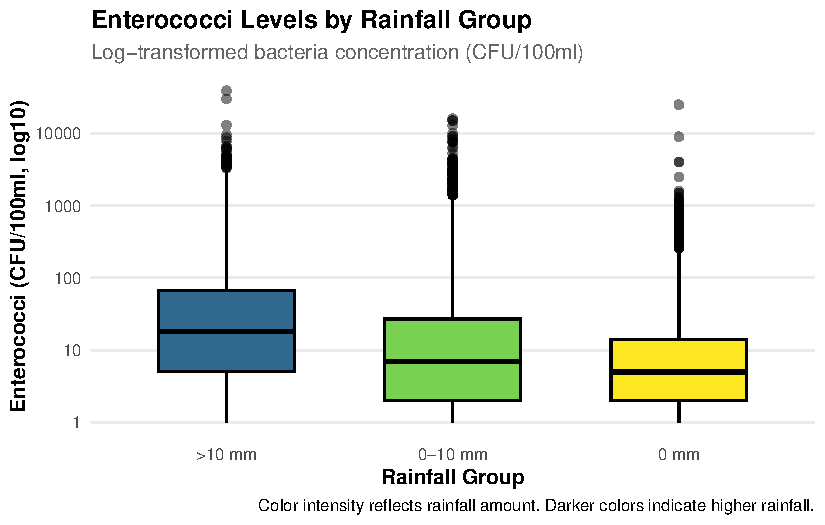
\includegraphics[keepaspectratio]{report-Jing_files/figure-pdf/fig-boxplot-1.pdf}}

}

\caption{\label{fig-boxplot}Boxplot of Enterococci Levels by Rainfall
Group}

\end{figure}%

\subsection{Result}\label{result}

From Figure~\ref{fig-bar_chart}, the beach with the highest average
pollution level is Wentworth Falls Lake - Jetty, with more than 500
CFU/100ml. This is about twice the level of the second-ranked site,
Megalong Creek. The other eight beaches in the top 10 also show high
pollution, at average values above 100 CFU/100ml. These results suggest
that certain beaches consistently have poor water quality from 2015 to
2025.

The Table~\ref{tbl-rain_table} shows that beaches with rainfall greater
than 10mm had significantly higher enterococci levels compared to those
with 0mm rainfall. It suggests a strong relationship between heavy
rainfall and increased bacteria concentration. The boxplot in
Figure~\ref{fig-boxplot} further supports this pattern. The
log-transformed enterococci levels are clearly higher in the
\textgreater10mm group. Besides, the entire box of \textgreater10mm
group is shifted upward, showing that rainfall likely plays a major role
in pollution spikes.

These findings are consistent with prior research that links high
bacteria levels with increased illness risk in swimmers, including
diarrhea and ear infections (Wade et al., 2012). Similar results were
found by Soller et al.~(2010), who showed that bacterial concentrations
tend to rise after heavy rainfall, increasing the likelihood of
gastrointestinal illness.

\subsection{Conclusion}\label{conclusion}

This study shows that some beaches in Sydney, such as Wentworth Falls
Lake - Jetty, have very high levels of enterococci. It can be dangerous
for public health because swimming in polluted water increases the risk
of getting sick, including diarrhea, ear infections and so on. The data
also show that rainfall has a strong influence on water quality. After
heavy rain, enterococci levels rise a lot. This means that rainfall is a
major reason why beach water becomes unsafe. Overall, the results
suggest that many beaches are not always safe for swimming, especially
after rain.

\subsection{Recommendations}\label{recommendations}

To protect public health, the government should test beach water quality
more often and make the results easy for the public to access. Warning
signs or online alerts can help people know when it is unsafe to swim.
It is especially important to avoid swimming after heavy rainfall. In
addition, weather forecasts and past data can help predict when beaches
are likely to be polluted. This can help create early warning systems
and reduce the risk of illness from swimming in dirty water.

\subsection{Reference}\label{reference}

Ackerman, D., \& Weisberg, S. B. (2003). Relationship between rainfall
and beach bacterial concentrations on Santa Monica Bay beaches. Journal
of water and health, 1(2), 85-89.

Colford, J. M., Jr, Schiff, K. C., Griffith, J. F., Yau, V., Arnold, B.
F., Wright, C. C., Gruber, J. S., Wade, T. J., Burns, S., Hayes, J.,
McGee, C., Gold, M., Cao, Y., Noble, R. T., Haugland, R., \& Weisberg,
S. B. (2012). Using rapid indicators for Enterococcus to assess the risk
of illness after exposure to urban runoff contaminated marine water.
Water research, 46(7), 2176--2186.
https://doi.org/10.1016/j.watres.2012.01.033




\end{document}
